\begin{figure}[h!]
    \centering
    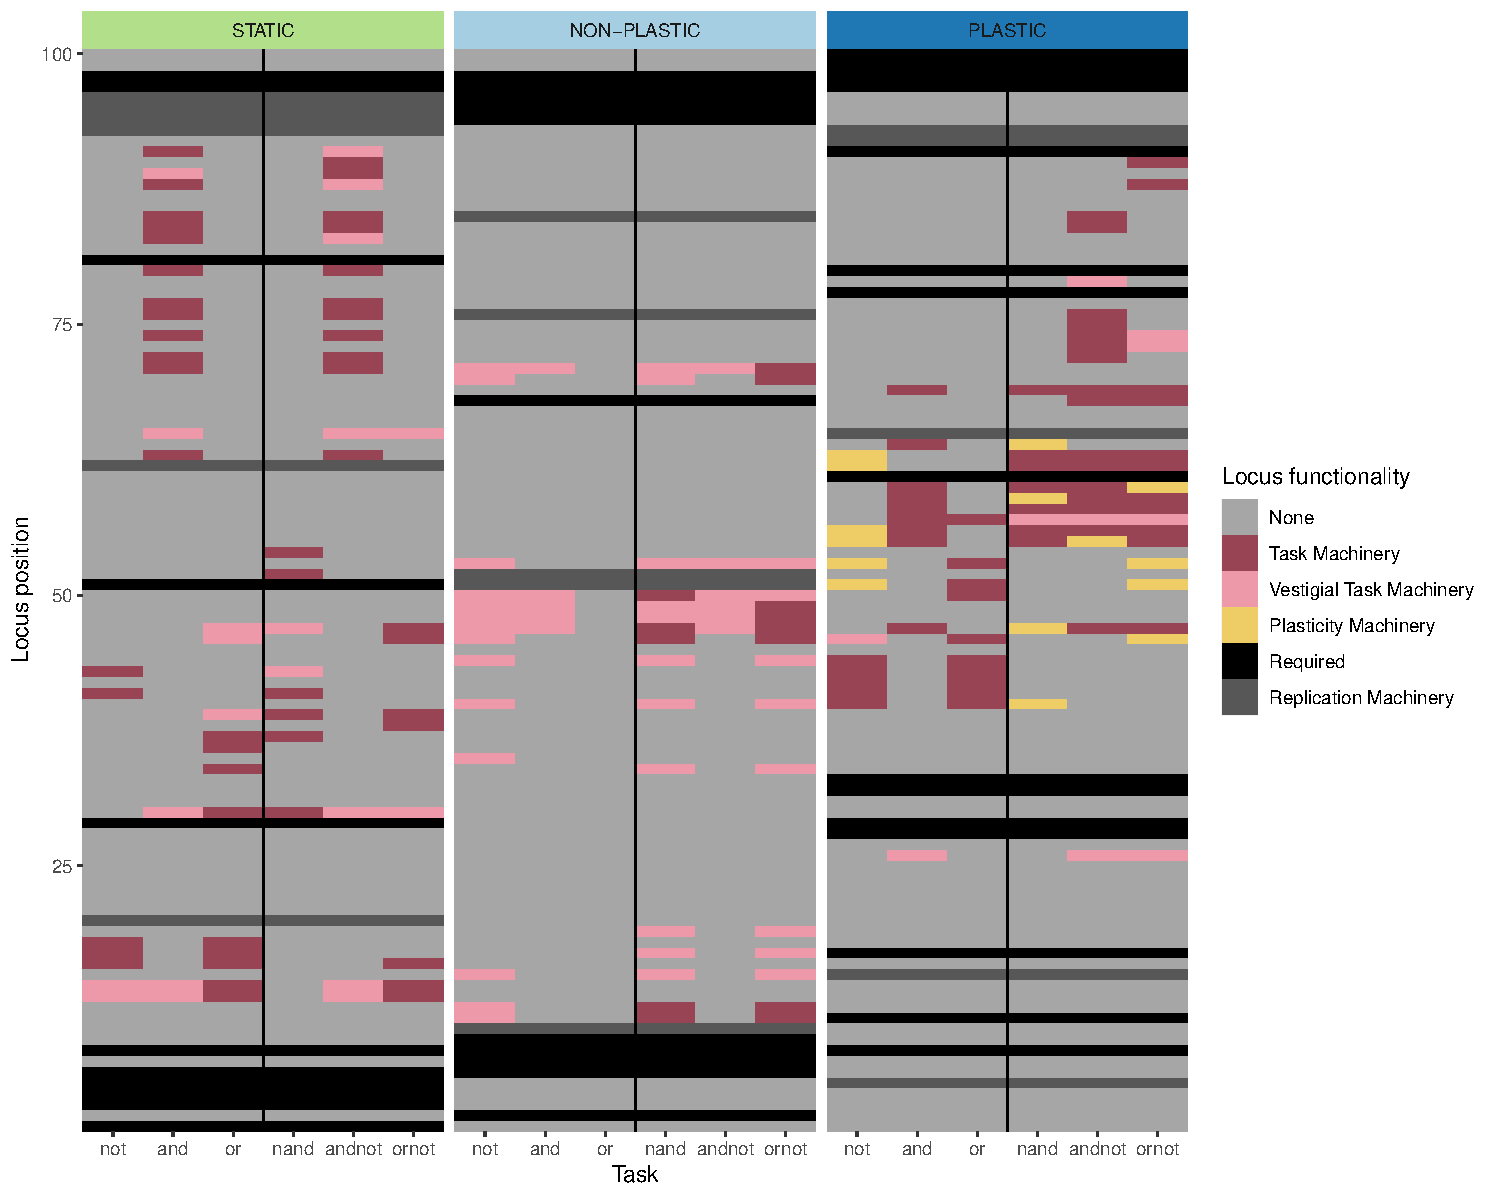
\includegraphics[width=1\textwidth]{media/architecture/locus_slice_combined_color_facets.pdf}
    \caption{\small
    % TODO: Change "Previous Task Machinery" -> "Vestigial Task Machinery"
    \textbf{Locus functionality.}
    Each box shows a representative genome from each condition at the end of Phase 2A. 
    The y-axis indicates each site in each genome, and colors indicate the function of each locus with respect to a particular task (given by the x-axis). 
    % Each of the six base tasks are shown on the x axis. 
    The vertical black line splits tasks rewarded in ENV-A (left of the line) from those rewarded in ENV-B.
    Loci colored as ``Task Machinery'' are actively involved in the performance of that task, while ``Vestigial Task Machinery'' represents loci that have not mutated, but no longer code for the task (\textit{i.e.}, a change elsewhere in the genome has disabled or modified the task). 
    ``Plasticity Machinery'' refers to loci that regulate the given task. 
    Knocking out a ``Replication Machinery'' locus negatively affects replication time, while knocking out a ``Required'' locus results in a non-viable organism. 
    }
    \label{fig:architecture_locus_functionality}
\end{figure}

% @AML: Original caption:
    % Each box shows a representative sample from each condition at the end of Phase 2A. 
    % The 100-loci genome of each sample is shown on the y axis, with colors indicating function of each locus has for each of the six base tasks. 
    % Each of the six base tasks are shown on the x axis. 
    % The vertical black line splits tasks rewarded in ENV-A (right of the line) from those rewarded in ENV-B.
    % Loci colored as Task Machinery are actively involved in the performance of that task, while Vestigial Task Machinery represents loci that have not mutated, but no longer code for the task (i.e., a change elsewhere in the genome has disabled or modified the task). 
    % Plasticity Machinery refers to loci that prevent the task from occurring in both the A and B environments. 
    % Knocking out a Replication Machinery locus will have a substantial negative effect on replication time, while knocking out a Required locus results in a non-viable organism. 
